\section{Experiments \& Evaluations}\label{results}

In this section, we will evaluate the performance of the online trajectory generation algorithms in simulation and in real robot table tennis experiments. We first start by comparing the ball returning performance of $\Alg$ ($\alg$) in simulation against the virtual hitting plane ($\vhp$) method. 

\subsection{Simulation Studies}\label{sim} %Comparison with the Virtual Hitting Plane method

In simulation the performance of the new table tennis players can be extensively evaluated without robot control and ball prediction errors. We will make controlled experiments to show that the player $\alg$ outperforms the $\vhp$ based player, and can generate striking trajectories more robustly.

\paragraph{\textbf{Virtual Hitting Plane Method}.} The VHP method that we implement is a close variant of \citet{Muelling11}. In this approach, the specification of the VHP (see Figure~\ref{vhps}) fixes the hitting time $\hitTime$ as well as the hitting point $\ballPred(\hitTime)$ for the racket trajectory. The remaining parameters, the desired racket velocity $\racketVel_{\mathrm{des}}(\hitTime)$ and the desired racket normal at hitting time $\normal_{\mathrm{des}}(\hitTime)$ are calculated by inverting the models~\eqref{flightModel} and \eqref{contactModel} at the hitting time $\hitTime$. 

%and \eqref{mirrorLaw} at the hitting time $\hitTime$. Unlike our more general approach in Section~\ref{calcDesRacket}, the inversion 
%
%\begin{align}
%v_{n}(\hitTime) = \frac{o_{n}(\hitTime) + \epsilon_R i_{n}(\hitTime)}{1 + \epsilon_{R}},
%\end{align}
%%
%results in the desired racket velocity along the normal $v_n$ and the desired normal. Racket velocity along the other two directions are fixed to zero to %minimize any accidental generation of spin. 

To run inverse kinematics (IK) on the desired hitting point, one needs to additionally specify a desired racket slide~\citep{Spong06}. An easy and convenient way to generate a desired racket slide at hitting time is to rotate the initial racket slide until the initial racket normal aligns with the final desired racket normal. This procedure determines the full orientation of the final robot posture at hitting time.

After specifying the orientation of the robot at hitting time, Jacobian pseudoinverse based IK can be run to determine the final joint positions. 
%To make IK more robust, we provide initial estimates from a lookup table. We look up the Cartesian and joint position values reached at the striking time estimates \eqref{strikingTimeEst} during our demonstrations. We can perform linear regression or interpolate between this demonstration data to quickly come up with good initial estimates. We then run a Jacobian pseduoinverse based IK algorithm on this initial estimate. 
IK typically takes less than $2$ ms to converge to $\joint_f$. Final joint velocities are then found by using the Jacobian at hitting time $\jac(\joint_f))$ and the desired racket velocities
%
\begin{align}
\dot{\joint}_f = \jac^{\dagger}(\joint_f)\racketVel_{\mathrm{des}}(\hitTime).
\end{align}
%
The computed parameters $\joint_f, \dot{\joint}_f$ along with the fixed hitting time $\hitTime$ fully determine a third degree polynomial in joint space for each degree of freedom of the robot $i = 1,\ldots,n$. The joint limitations are then checked and the procedure is repeated if the accelerations are too high. When the ball is coming close to the robot's initial posture $\joint_0$, this complicated IK procedure results in feasible trajectories if the VHP is chosen appropriately. However, it is rather inflexible and can easily fail to find good configurations. 
%the Cartesian constraints due to the table. 
%The actual joint limits for the Barrett WAM are shown in Table~\ref{joint limits} in the appendix. 
% TODO: talk more about IK? ref needed 

\paragraph{\textbf{Comparison with the VHP Method}.} To make a fair comparison between the $\vhp$ approach and our algorithm $\alg$, in our simulation environment\footnote{Code for the simulation platform as well as a video showing some example trajectories is available in the GitHub repository: https://github.com/RobotLearning/traj-gen-and-tracking.git} the initial ball state variance is fixed such that most balls end up close to the initial robot posture. This ensures that a fair evaluation between the two algorithms can be given. Both methods filter the incoming stream of ball position estimates using the same Extended Kalman Filter (EKF) and equally start moving whenever $N \approx 5$ balls are detected. 
%If this value is less than $T_{\mathrm{max}} = 0.6$ sec, trajectory generation is launched. This occurs generally after the ball passes the net.

\begin{table}[b!]
\small\sf\centering
\renewcommand{\arraystretch}{1.3}
\caption{Results comparing $\alg$ and $\vhp$}
\label{tableSimResults}
\begin{tabular}{c||c|c|c|c}
\toprule
& {\small \bfseries Returns} & {\small \bfseries Not Valid} & {\small \bfseries Infeasible} & {\small \bfseries Miss/Out} \\
\hline
{\small $\alg$} & 151 & 24 & 19 & 6\\
\hline
{\small $\vhp$} & 125 & 24 & 45 & 6\\
\bottomrule
\end{tabular}
\end{table}
%
\begin{figure}[t!]
\centering
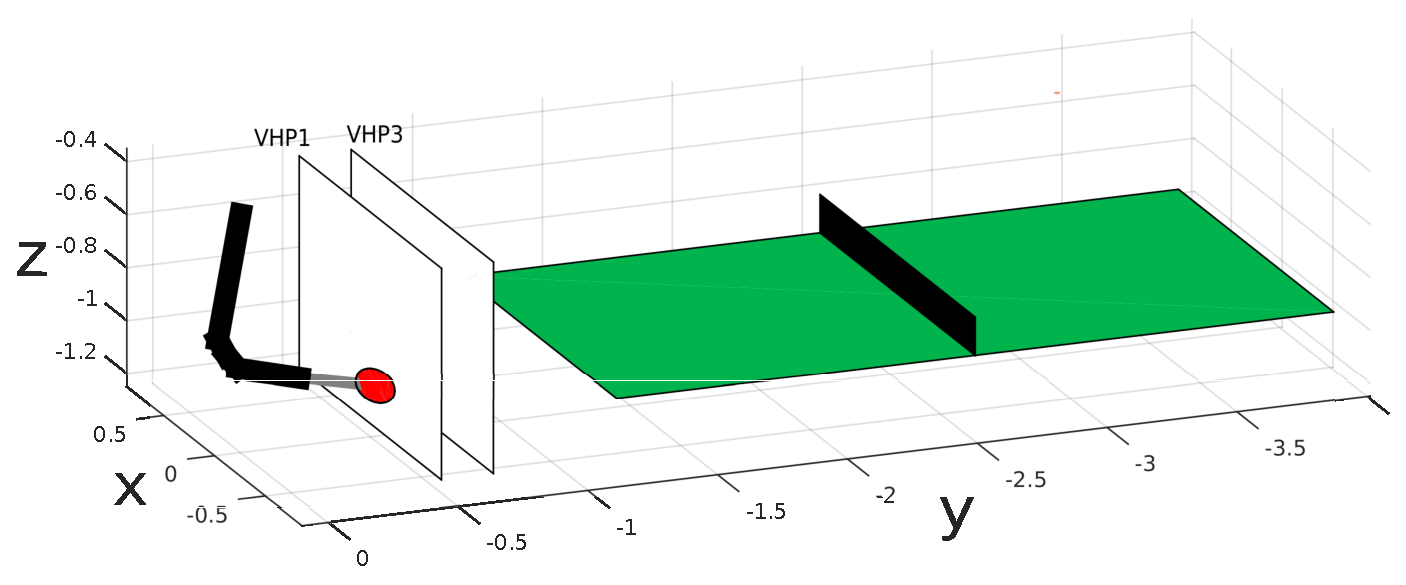
\includegraphics[scale=0.3]{tableTennisVHP.eps}
\caption{For simulating the performance of the virtual hitting plane (VHP) based method in a fair way, the results are averaged over four different VHP locations. The first and third plane locations are shown in the figure. Out of $50$ balls each, the VHP at $y=\mbox{-}0.7$, $y=\mbox{-}0.6$, $y=\mbox{-}0.5$, $y=\mbox{-}0.4$ return $31, 37, 28, 29$ balls respectively.}
\label{vhps}
\end{figure}
%
Evaluations are summarized in Table~\ref{tableSimResults}. A total of $200$ balls are launched towards the robot in single-ball solo trials from varying initial positions and velocities, $\ball_{\mathrm{init}} \sim \mathcal{N}(\vec{\mu}_{\mathrm{init}}, \sigma_{\mathrm{init}}^2 \vec{I})$. The initial ball mean positions are fixed on the left corner of the opponent's court and the initial covariance matrix is diagonal with a standard deviation of $\sigma_{\mathrm{init}} = 0.1$. Some balls are illegal, for example they might not bounce on the robot's court. Such balls are detected with our ball prediction models and they are not considered for strike generation. They are marked as \emph{Not Valid} in Table~\ref{tableSimResults}. 

Comparing with the VHP method, it can be seen that $\alg$ is able to return more balls to the other side, with $26$ more balls returned to the opponent's court. One of the main reasons for this increase in performance is the fixed location of the VHP. Depending on the incoming ball velocity, trajectories generated using a fixed VHP can result in joint limit violations or infeasible solutions. They are marked as \emph{Infeasible} in Table~\ref{tableSimResults}. A second reason is the explicit incorporation of joint limits both for the striking trajectory and the returning trajectory in the optimization problem. See Figure~\ref{vhps} for an illustration. Out of $50$ balls each, the VHP methods with the planes fixed at $y=\mbox{-}0.7$, $y=\mbox{-}0.6$, $y=\mbox{-}0.5$, $y=\mbox{-}0.4$ locations return $31, 37, 28, 29$ balls respectively. For this particular ball distribution, the plane at $y = \mbox{-}0.7$ seems to be the most robust option.

\paragraph{\textbf{Lookup Table}.} A naive implementation of $\alg$ in MATLAB using Sequential Quadratic Programming (SQP), takes about two seconds on our system on average. \citet{Koc16} proposed a lookup table as a remedy to replace online optimization. Whenever a strike computed offline is successful in returning the ball in simulation, ball positions, velocities at the start of the movement and the optimized parameters $\, \joint_f, \dot{\joint}_f, T$ can be stored in a lookup table. One can then at runtime simply lookup the optimized parameters that have the closest stored ball position and velocity estimates to new ball estimates. The performance of this lookup table based approach is evaluated in Figure~\ref{fig:offline}. The same initial ball distribution with the same $\vec{\mu}_{\mathrm{init}}, \sigma_{\mathrm{init}}$ values is used as before. As the number of lookup table samples increase, the percentage of incoming balls returned successfully approaches that of the online trajectory generation. 

The simple lookup table approach that is employed here corresponds to k-nearest neighbor interpolation with $k = 1$. Machine learning based methods that regress between lookup table entries using more sophisticated approaches are discussed extensively in, for example, \citet{Lampariello11}.

\begin{figure}[t!]
\centering
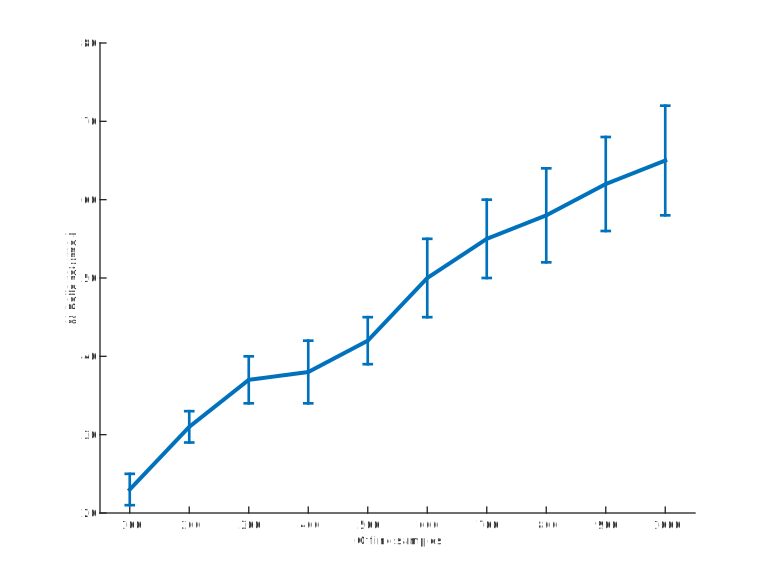
\includegraphics[scale=0.22]{offline.pdf}	
\caption{As an alternative to computing the trajectory parameters online, \citet{Koc16} proposed a lookup table to generate trajectories. Performance of the trajectory generation framework using a lookup table is shown in blue. Results are averaged over $5$ different runs. As the number of stored lookup table samples increase, the performance approaches that of the online trajectory generation in (a). However, as shown in (b), even the performance of a lookup table with $4000$ entries degrades quickly whenever ball position and velocity estimates are not close to the values stored in the lookup table. }
\label{fig:offline}
\end{figure}

\paragraph{\textbf{Online Trajectory Generation}.} The lookup table proposed above is based on a fixed initial posture $\joint_{0}$ while the robot is at rest, i.e., $\dot{\joint}_0 = \vec{0}$. Its performance degrades whenever filtered ball positions $\ball_0$ and velocities $\dot{\ball}_0$ are not close to the values stored in the lookup table, or when the initial posture is different. See Figure~\ref{fig:offline} for the decrease in performance of a lookup table with $4000$ entries, as the mean of the initial ball distribution, $\vec{\mu} \sim \mathcal{N}(\vec{\mu}_{\mathrm{init}},\sigma^{2}\vec{I})$, is randomized with increasing variances $\sigma^{2}$. %ball state estimate and trajectory parameter 

To overcome the shortcomings of a lookup-table based approach, we implemented the optimizations in $\CC$ with an interface to the simulation environment SL~\citep{Schaal06}\footnote{$\CC$ code for the online optimization run in the real-time simulation platform SL can be found in: https://github.com/RobotLearning/polyoptim.git.}. SL is also our real-time interface to the robot and runs at a frequency of $500$ Hz, terminating any processes that do not finish within $2$ milliseconds. It is mainly responsible for running the inverse dynamics and feedback control loop computations. To run the optimization online, a thread separate from the one running the inverse dynamics is launched, whenever there are reliable ball observations available and another thread is not running.

We use the NLopt library~\citep{NLopt} to run the optimizations. We found that among the nonlinear constrained optimization routines, only COBYLA respects the equality constraints given in \mbox{\eqref{transCond1} -- \eqref{transCond3}} for the $\Alg \ (\alg)$. The algorithm COBYLA is a simplex method implemented in NLopt that uses direct search with linear approximations~\citep{Powell94}. Gradients of the cost function~\eqref{costFnc3} can be easily calculated and fed to a gradient based solver, but this direct search routine takes only about $20$ ms to converge, i.e., about the same frequency as the incoming ball observations. For the $\AlgTwo \ (\algTwo)$, the Augmented Lagrangian (AUGLAG) method is used to convert the problem to an unconstrained optimization problem, which is then solved with a Quasi-Newton algorithm, taking on average about $25$ ms to converge. 

Good initialization does not always guarantee faster convergence, but it can help escape bad local minima of the cost functions. The optimization parameters for $\alg$ are first initialized to the current resting posture, $\joint_f = \joint_0, \ \dot{\joint}_f = \vec{0}$ and $\hitTime = 0.5$. Whenever the robot is already moving and corrections are being computed, the parameters are initialized to their previously computed values. For $\algTwo$, we regress on a lookup table using k-nearest-neighbor (kNN) regression, with $k = 5$, to initialize the optimization variables.

\paragraph{\textbf{Online Corrections}.} In order to show the performance increase due to online corrections, we first put Gaussian white noise with $\sigma = 0.02 $ m standard deviation on the ball observations and apply Extended Kalman Filter (EKF). As the ball approaches, the robot gets increasingly better estimates of the ball state. Our real-time simulator runs at $500$ Hz, while the ball observation is limited to $60$ Hz, limiting the frequency of online corrections.
%
\begin{figure}[t]
	%\centering
	\setlength\figureheight{3cm}
	\subcaptionbox{Performance under ball observation noise\label{players-obs-noise}}{
		\setlength\figurewidth{3cm}
		% This file was created by matlab2tikz.
%
%The latest updates can be retrieved from
%  http://www.mathworks.com/matlabcentral/fileexchange/22022-matlab2tikz-matlab2tikz
%where you can also make suggestions and rate matlab2tikz.
%
\definecolor{mycolor1}{rgb}{0.20810,0.16630,0.52920}%
\definecolor{mycolor2}{rgb}{0.21783,0.72504,0.61926}%
\definecolor{mycolor3}{rgb}{0.97630,0.98310,0.05380}%
%
\begin{tikzpicture}

\begin{axis}[%
width=0.951\figurewidth,
height=\figureheight,
at={(0\figurewidth,0\figureheight)},
scale only axis,
bar width=0.8,
xmin=0.5,
xmax=3.5,
xtick={1,2,3},
xticklabels={{FP},{DP},{VHP}},
ymin=0,
ymax=145,
axis background/.style={fill=white},
axis x line*=bottom,
axis y line*=left
]
\addplot[ybar stacked, fill=mycolor1, draw=black, area legend] table[row sep=crcr] {%
1	123\\
2	0\\
3	0\\
};
\addplot[forget plot, color=white!15!black] table[row sep=crcr] {%
0.5	0\\
3.5	0\\
};
\addplot[ybar stacked, fill=mycolor2, draw=black, area legend] table[row sep=crcr] {%
1	0\\
2	130\\
3	0\\
};
\addplot[forget plot, color=white!15!black] table[row sep=crcr] {%
0.5	0\\
3.5	0\\
};
\addplot[ybar stacked, fill=mycolor3, draw=black, area legend] table[row sep=crcr] {%
1	0\\
2	0\\
3	106\\
};
\addplot[forget plot, color=white!15!black] table[row sep=crcr] {%
0.5	0\\
3.5	0\\
};
\node[right, align=left]
at (axis cs:0.649,130.045) {123};
\node[right, align=left]
at (axis cs:1.632,138.182) {130};
\node[right, align=left]
at (axis cs:2.616,114.409) {106};
\end{axis}
\end{tikzpicture}%
	}\hfill%\hspace{1em}
	\subcaptionbox{Performance under additional ball model mismatch\label{players-mismatch}}{
		\setlength\figurewidth{3cm}
		% This file was created by matlab2tikz.
%
%The latest updates can be retrieved from
%  http://www.mathworks.com/matlabcentral/fileexchange/22022-matlab2tikz-matlab2tikz
%where you can also make suggestions and rate matlab2tikz.
%
\definecolor{mycolor1}{rgb}{0.20810,0.16630,0.52920}%
\definecolor{mycolor2}{rgb}{0.21783,0.72504,0.61926}%
\definecolor{mycolor3}{rgb}{0.97630,0.98310,0.05380}%
%
\begin{tikzpicture}

\begin{axis}[%
width=0.951\figurewidth,
height=\figureheight,
at={(0\figurewidth,0\figureheight)},
scale only axis,
bar width=0.8,
clip=false,
xmin=0.5,
xmax=3.5,
xtick={1,2,3},
xticklabels={{FP},{DP},{VHP}},
ymin=0,
ymax=140,
axis background/.style={fill=white},
axis x line*=bottom,
axis y line*=left
]
\addplot[ybar stacked, fill=mycolor1, draw=black, area legend] table[row sep=crcr] {%
1	124\\
2	0\\
3	0\\
};
\addplot[forget plot, color=white!15!black] table[row sep=crcr] {%
0.5	0\\
3.5	0\\
};
\addplot[ybar stacked, fill=mycolor2, draw=black, area legend] table[row sep=crcr] {%
1	0\\
2	140\\
3	0\\
};
\addplot[forget plot, color=white!15!black] table[row sep=crcr] {%
0.5	0\\
3.5	0\\
};
\addplot[ybar stacked, fill=mycolor3, draw=black, area legend] table[row sep=crcr] {%
1	0\\
2	0\\
3	53\\
};
\addplot[forget plot, color=white!15!black] table[row sep=crcr] {%
0.5	0\\
3.5	0\\
};
\node[right, align=left]
at (axis cs:0.624,131.032) {124};
\node[right, align=left]
at (axis cs:1.608,147.079) {140};
\node[right, align=left]
at (axis cs:2.681,60.444) {53};
\end{axis}
\end{tikzpicture}%
	}%
	\caption{Simulation results comparing the returns of three table tennis players. In (a), ball positions are observed with Gaussian white noise. In (b), there is an additional mismatch due to unknown topspin. Out of $200$ balls, $14$ and $12$ incoming balls did not bounce legally and were not considered for trajectory generation, respectively. The other balls that were not counted as returns were either missed, or did not land legally on the opponent's court.}
	\label{compare-players-sim}
\end{figure}
%
The results are summarized in Figure~\ref{players-obs-noise}, averaged over three different ballgun locations: center, right and left. The initial pose of the robot is placed opposite accordingly, i.e. on the right side of the table if the ball is coming from the left. Out of $200$ balls, $14$ incoming balls did not bounce legally and were not considered for trajectory generation. The other balls that were not returned successfully were either missed, or did not land legally on the opponent's court. The online optimization is started whenever there are $\numBallsMin = \minball$ ball samples available. This is enough to ensure that the estimated ball velocities will not cause robot movements that are far off from the ball. The solver then continues at a rate of $25$ Hz until the ball appears behind the racket centre, i.e., $b_y > r_y$. Any ball that suddenly appears on the opponent's court causes the Kalman Filter to reset, reinitialized with that ball observation as the initial mean and with a high variance.

The players that generate trajectories only once are able to return only very few balls ($10$ on average) in this mode of evaluation. Correcting with the $\vhp$ method improves the returning performance significantly. However, balls that are not feasible for the robot in the Virtual Hitting Plane intersection cannot be returned at all with this player. $\Alg$ ($\alg$) and $\AlgTwo$ ($\algTwo$) on the other hand, can find and generate feasible movements more flexibly.

As an additional challenge, we also consider the model mismatch case where there is a very high topspin on the ball, around $3000$ revolutions per minute (rpm). EKF assumes a nonspinning model for the ball, i.e., $\lift = 0$. The solver is run with an increased rate of $50$ Hz to be able to return the balls. The players that generate trajectories only once are not able to return any balls in this aggressive mode of evaluation. The results are summarized in Table~\ref{players-mismatch}.$\ 14$ incoming balls out of $200$ did not bounce legally and were not considered for trajectory generation. As in the previous experiment, $\alg$ and $\algTwo$ corrects the trajectories more easily and overall return more balls. The advantage of $\algTwo$ over $\alg$ in this setting is due to the more flexible returning criterion, as the resting state optimization was not applied.